\pgfplotsset{compat=1.12}
\pgfplotsset{every tick label/.append style={font=\scriptsize}}
  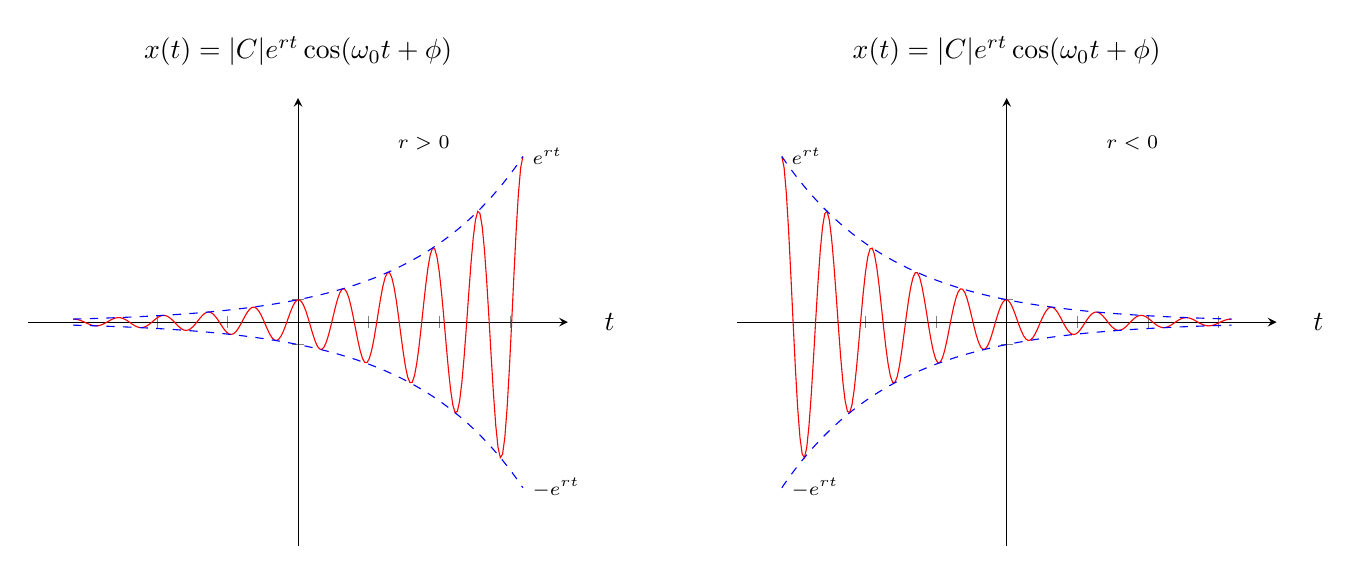
\begin{tikzpicture}
  \def\omwga0{2*pi}
  \def\phase{-45}
  \def\r{0.4}
    \begin{axis}[
     clip=false,
     xmin=-6,xmax=6,
     xlabel= $t$,
     ylabel={$x(t)=|C|e^{rt}\cos(\omega_0t+\phi)$},
     ymin=-10,ymax=10,
     axis lines=middle,
     %axis x line=middle,
     %axis y line=left,
%     axis x line=middle,
     xtick={-3.14, -1.57, 0,1.57,3.14,4.71,6.28, 7.85},
     %xticklabels={$-\pi$, $-\frac{\pi}{2}$, $0$, $\frac{\pi}{2}$,$\pi\,$,$\,\,\,\frac{3}{2}\pi$,$\,\,\,2\pi$, $\frac{5\pi}{2}$},
     xticklabels=\empty,
     ytick={-1, 1},
     yticklabels=\empty,
     %xticklabel style={anchor=north west}
     every axis x label/.style={
    at={(ticklabel* cs:1.05)},
    anchor=west,
},
every axis y label/.style={
    at={(ticklabel* cs:1.05)},
    anchor=south,
},
     ]
      \addplot[domain=-5:5,samples=200,red]{exp(\r*x)*cos(2*pi*deg(x))};
      \addplot[domain=-5:5,samples=200,blue, dashed]{exp(\r*x)}
                                node[right,pos=1,font=\footnotesize, black]{\scriptsize $e^{rt}$};       
                                      \addplot[domain=-5:5,samples=200,blue, dashed]{-exp(\r*x)}
                                node[right,pos=1,font=\footnotesize, black]{\scriptsize $-e^{rt}$};               
       \node at (axis cs:2, 8) [anchor=west] {\scriptsize $r>0$ };
    \end{axis}
    
    
    \begin{scope}[xshift=9cm]

  \def\omwga0{2*pi}
  \def\phase{-45}
  \def\r{-0.4}
    \begin{axis}[
     clip=false,
     xmin=-6,xmax=6,
     xlabel= $t$,
     ylabel={$x(t)=|C|e^{rt}\cos(\omega_0t+\phi)$},
     ymin=-10,ymax=10,
     axis lines=middle,
     %axis x line=middle,
     %axis y line=left,
%     axis x line=middle,
     xtick={-3.14, -1.57, 0,1.57,3.14,4.71,6.28, 7.85},
     %xticklabels={$-\pi$, $-\frac{\pi}{2}$, $0$, $\frac{\pi}{2}$,$\pi\,$,$\,\,\,\frac{3}{2}\pi$,$\,\,\,2\pi$, $\frac{5\pi}{2}$},
     xticklabels=\empty,
     ytick={-1, 1},
     yticklabels=\empty,
     %xticklabel style={anchor=north west}
     every axis x label/.style={
    at={(ticklabel* cs:1.05)},
    anchor=west,
},
every axis y label/.style={
    at={(ticklabel* cs:1.05)},
    anchor=south,
},
     ]
      \addplot[domain=-5:5,samples=200,red]{exp(\r*x)*cos(2*pi*deg(x))};
      \addplot[domain=-5:5,samples=200,blue, dashed]{exp(\r*x)}
                                node[right,pos=0,font=\footnotesize, black]{\scriptsize $e^{rt}$};       
                                      \addplot[domain=-5:5,samples=200,blue, dashed]{-exp(\r*x)}
                                node[right,pos=0,font=\footnotesize, black]{\scriptsize $-e^{rt}$};               
       \node at (axis cs:2, 8) [anchor=west] {\scriptsize $r<0$ };
    \end{axis}
   
	\end{scope}


  \end{tikzpicture} 